\section{Design API Rest}
\subsection{Description}

\begin{flushleft}
Afin d'interagir entre le l'application et la base de données, des requêtes sont envoyées via l'API Rest permettant cette communication. C'est pourquoi certains services ont été ajoutés à la base commune de l'API.
Pour les mêmes raisons que la partie commune, le token de connexion est repris à chaque fois
\end{flushleft}

\begin{flushleft}
Pour qu'un client puisse voir la liste de ses factures, une requête "GET" doit être envoyée. Dans cette requête, un paramètre "id_facture" est nécessaire pour voir une facture en particulier. Si ce paramètre vaut "NULL", toutes les factures sont affichées.
Cette requête renvoie donc un objet "Facture" comprenant les même éléments cités précédemment.
\end{flushleft}

\begin{flushleft}
Un client peut modifier l'acompte proposé par l'application. C'est pourquoi, une requête "PUT" peut être envoyée contenant un paramètre "account" spécifiant la nouvelle valeur de l'acompte.
De la même manière, les informations de paiement et informations bancaires peuvent être modifiées à l'aide du même type de requête.
Il faut cependant noter que le paramètre "id_facture" ne peut plus être "NULL" sous peine de générer une erreur.
\end{flushleft}

\begin{figure}[h]
\subsection{Schéma}
\centering
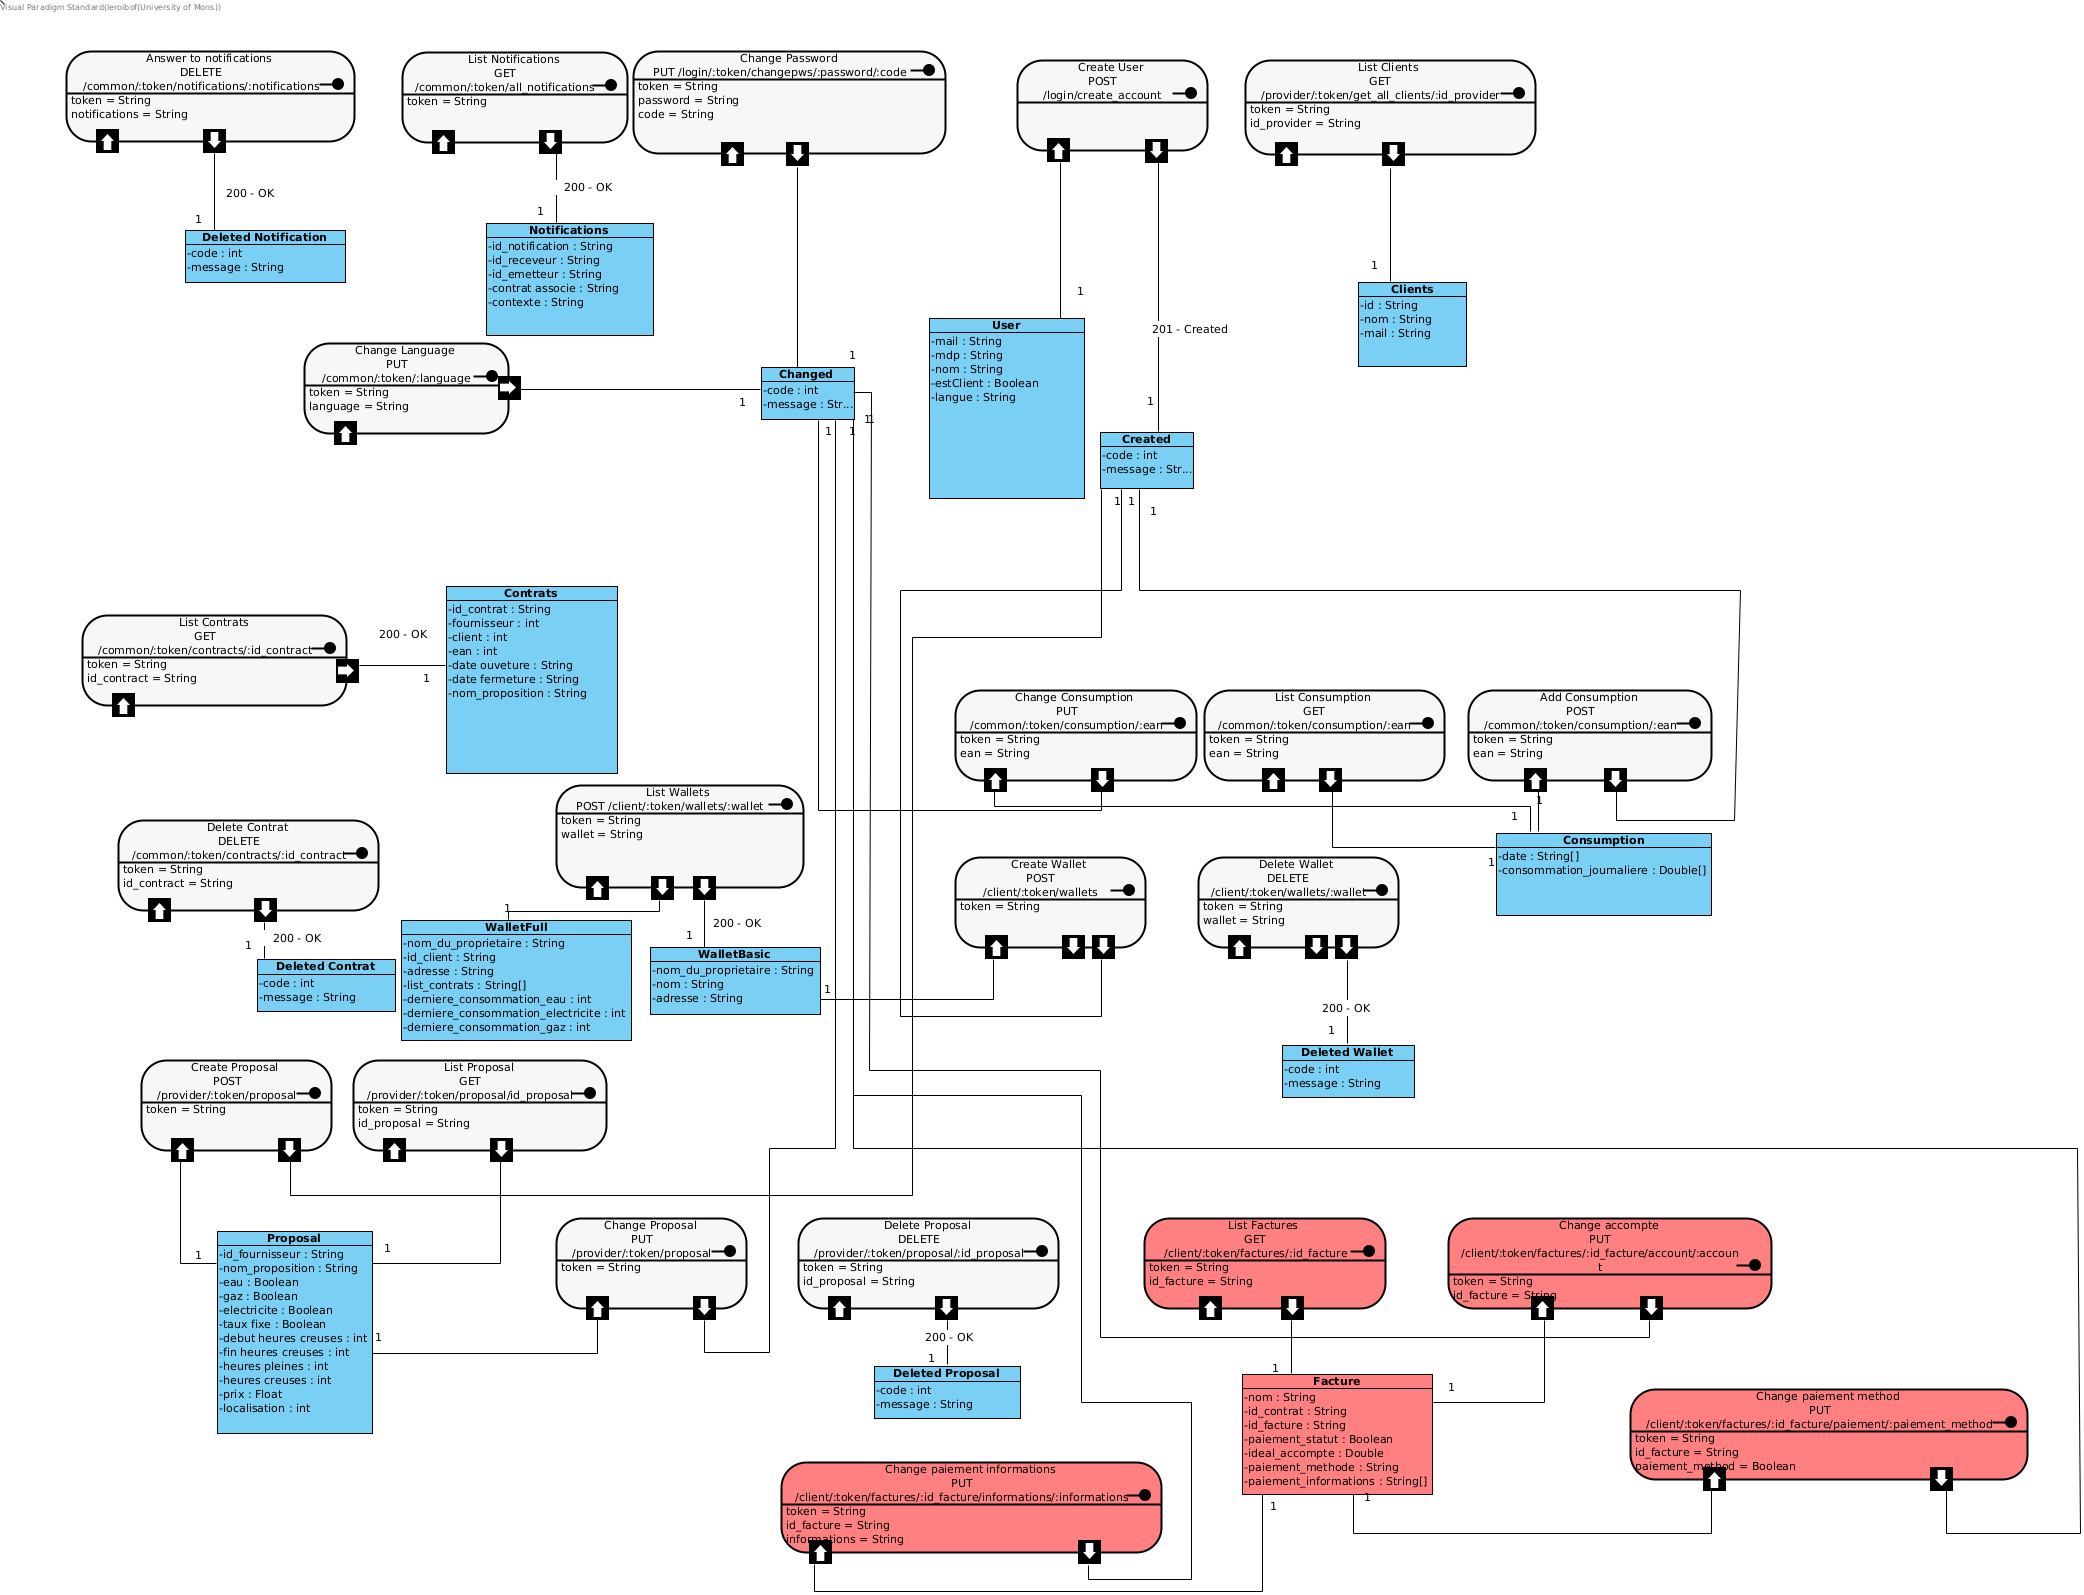
\includegraphics[width = 1\textwidth]{extension-maxime/apirest/img/apirest-extension.png}
\end{figure}
